\documentclass[12pt,a4paper]{jbook}
\usepackage{mm-thesis}
\usepackage[dvipdfmx]{graphicx}
\usepackage{cite}
\usepackage{comment}
\usepackage{docmute}
\usepackage{color}
\usepackage{moreverb}
\usepackage{listings}
\usepackage{ascmac}
%\usepackage{amsmath}
%\usepackage{amsthm}
%\usepackage{amsfonts}

\lstset{
	%枠外での自動改行
 	breaklines = true,
 	%標準の書体
 	basicstyle = {\small},
 	%枠 "t"は上に線を記載, "T"は上に二重線を記載
	%他オプション:leftline,topline,bottomline,lines,single,shadowbox
 	frame = TB,
 	%タブの大きさ
 	tabsize = 2,
 	%キャプションの場所("tb"ならば上下両方に記載)
 	captionpos = t,
 	%行番号の位置
 	numbers = left,
 	%自動改行後のインデント量(デフォルトでは20[pt])	
 	breakindent = 30pt,
	%左右の位置調整 	
 	xleftmargin=30pt,
 	xrightmargin=30pt,
	%プログラム言語(複数の言語に対応,C,C++も可)
 	%language = Python, 	
 	%背景色と透過度
 	%backgroundcolor={\color[gray]{.90}},
 	%コメントの書体
 	%commentstyle = {\itshape \color[cmyk]{1,0.4,1,0}},
 	%関数名等の色の設定
 	%classoffset = 0,
 	%キーワード(int, ifなど)の書体
 	%keywordstyle = {\bfseries \color[cmyk]{0,1,0,0}},
 	%表示する文字の書体
 	%stringstyle = {\ttfamily \color[rgb]{0,0,1}},
 	%frameまでの間隔(行番号とプログラムの間)
 	%framesep = 5pt,
 	%行番号の間隔
 	%stepnumber = 1,
	%行番号の書体
 	%numberstyle = \tiny,
}
\renewcommand{\lstlistingname}{Code}
\begin{document}
\newpage

\chapter{Alloyにおける時相論理の記述法の提案}
\label{sec:ProposedModel-TemporalLogic}
この章では、イベント発生時におけるウェブの様々な要素の状態変化の表現に利用可能なAlloyでの時相論理の記述法を提案する。

前述の\ref{sec:existing-models-problems}節における既存モデルの時相論理の表現能力の問題点は、「時間軸全体を通して状態変化を捉えることができない」ことである。
そもそも、Cookieモデルにおいて、状態クラス(CookieモデルにけるCSStateクラス)間の関係性はTransactionクラスのみ用いて表現している。
これが要因となり、同一のTransaction内での状態変化のみの表現能力となっている。
したがって、状態クラス間の関係性をTransactionに因らない記述法で表現することが必要となる。
また、CookieモデルにおけるCSStateクラスはCookieの状態を表現するためのクラスであり、CSStateのみに利用できる記法では、他のウェブの要素に応用できず汎用性の低い成果となる。
以上より、本研究では様々なウェブの要素の状態を表現できる汎用的なクラスを定義し、それらのクラスに統一して利用できる述語を提案する。

ここで、時間軸全体を通して状態変化を表現するためにどのような述語が必要となるかを考える。
まず、ある二状態に対してそれらが時間軸上で連続しているかを判定できれば、
「前後の二状態で起こりうる変化」を表現可能になる。
これに加えて状態遷移の初期状態を判定できれば、「初期状態にかかる条件(初期条件)」を表現可能になる。
これら二つの表現能力を組み合わせることで、帰納的に時間軸全体で起こりうる状態変化を表現可能となる。
以上より、時間軸全体での状態変化を表現するために以下の述語を作成する。
\begin{itemize}
\item 状態遷移において、直前にあたる状態を判定する述語
\item 初期状態を判定する述語
\end{itemize}

また、本記述法を用いる上で基礎モデルでの時間軸の表現(\ref{sec:based-model-temporal-logic}節参照)を一部変更している。
その変更点についても以降で述べる。

\section{時間軸の表現の変更}
基礎モデル\cite{based-model}においては、時間軸を表すTimeクラスにネットワーク上で発生するレスポンスやリクエストを表すEventクラスが関連付けられている。
これらのクラス間の関係性は、「ある時点Time0とTime1の間でEvent0が発生した」といった内容を表現できるものであり、二つのTimeクラスのインスタンスで一つのイベントの時刻を表現できる。
この関係性はEventのみが時間軸に関連付けられていたために利用できた。

これに対し、本提案記述法ではEventクラスに加えて、ある時点におけるウェブの要素の状態を表すStateクラスも時間軸に関連付けられる。
ここで、二つのTimeクラスのインスタンスで一つのイベントの時刻を表現するという既存モデルの関係性を維持すると、導入する述語の論理式が複雑となり実装が困難となる。
したがって、本提案モデルでは図\ref{fig:ProposedModel-TimeClass}に示す、一つのTimeクラスのインスタンスでイベントの時刻を表現できる記述法に変更する。

\begin{figure}[htb]
\centering
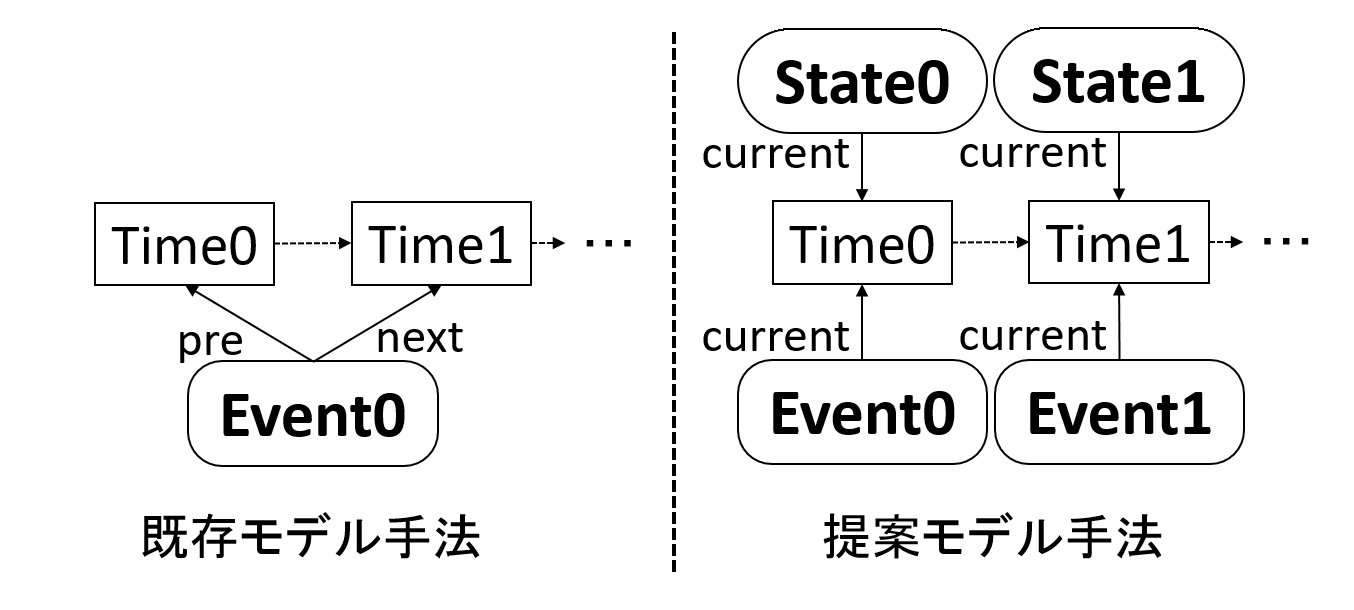
\includegraphics[width=450pt]{./fig/ProposedModel-TimeClass.eps}
\caption{提案モデルにおける時間軸とイベントの関係}
\label{fig:ProposedModel-TimeClass}
\end{figure}

この表現の変更によって、二つの既存モデルそれぞれにおける時相論理の表現能力に変更はない。
そもそも基礎モデルにおいて、二つのTimeクラスのインスタンスを利用する関係性を採用した理由は今後の拡張性を想定したためである。
基礎モデルには「リクエストやレスポンスといったイベントが同時刻で発生しない」といった制限が存在しており、このようなTimeクラスの関係性を用いていた場合には、この制限を取り払う拡張が容易となると考えられていた。
しかし、表現の変更後も同様に制限を取り除く拡張は可能である。
つまり、この変更によって既存モデルの表現能力と拡張性を妨げることはない。

\section{汎用的な状態クラス}
\label{sec:state-class}
導入する状態クラスとしてCode\ref{code:StateClass}に示すStateクラスを定義する。
flowはStateクラス同士を接続し状態の遷移を、currentはその状態となり得る時刻を表す。
また、その他の項目としてEqItem、DifItemクラスをStateクラスの変数としている。
\begin{lstlisting}[caption=Stateクラス, label=code:StateClass]
abstract sig State{
	flow: set State,
	eq: one EqItem,
	dif: one DifItem,
	current: set Time
}
abstract sig EqItem{}
abstract sig DifItem{}
sig StateTransaction extends HTTPTransaction{
	beforeState: set State,
	afterState: set State
}
\end{lstlisting}

まず、EqItemは同一の状態遷移上で変化しない要素(以下、「不変項目」とする)を表すクラスである。
不変項目は複数のStateが存在する場合に、いずれのStateが同一の遷移であるのかを判定するために用いる。
例えばStateが三つ存在している場合を考えると、図\ref{fig:ProposedModel-3StateFlow}に挙げられるように複数の遷移のパターンが考えられる。
ここで、EqItemをStateごとに比較をすることで、同一のEqItemを持つStateを同一の遷移に存在すると判定することができる。
図\ref{fig:ProposedModel-3StateFlow}を例にとると、三状態が同一の遷移に存在する場合にはState0,1,2のEqItemがすべて同一となる。
一方で、三状態が同一の遷移に存在しない場合にはState0,2のEqItemが同一であり、State1のEqItemはそれらと異なる値をとる。

\begin{figure}[htb]
\centering
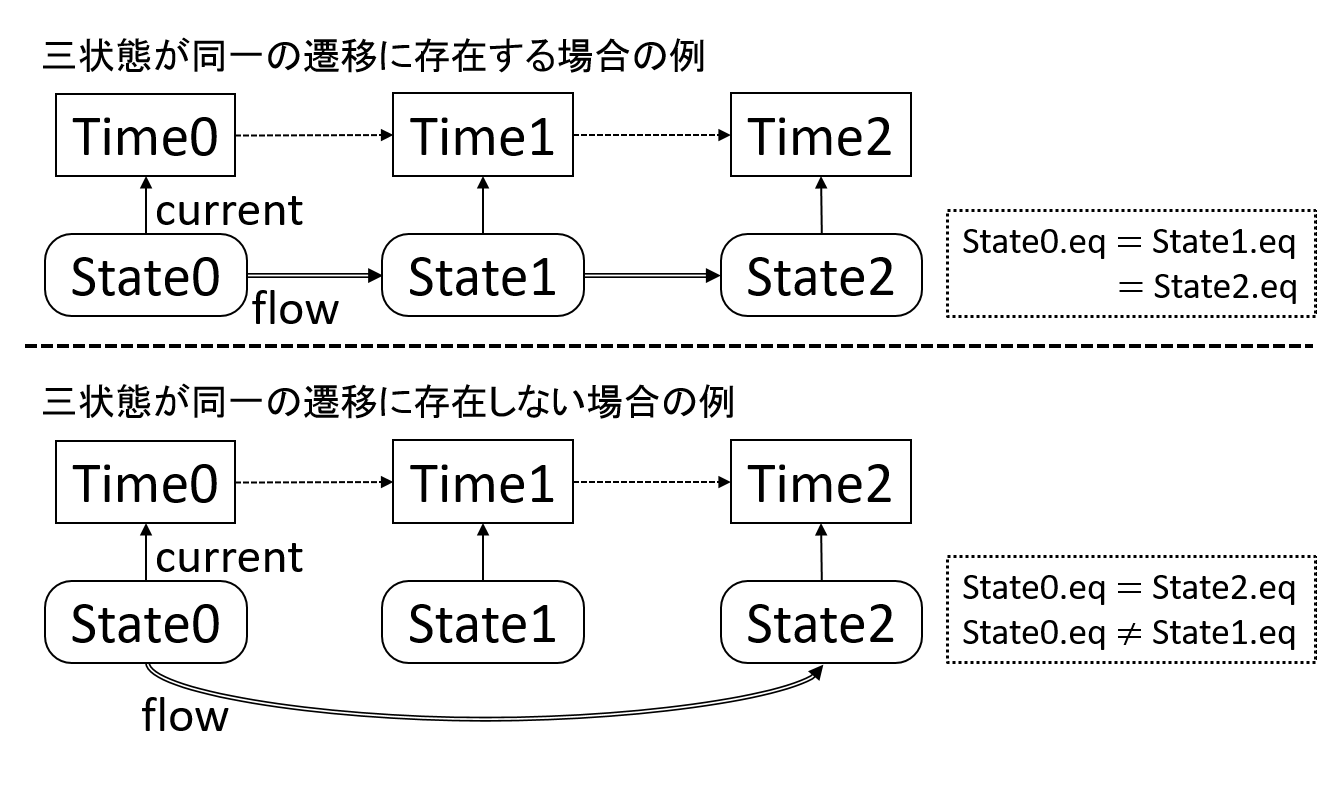
\includegraphics[width=400pt]{./fig/ProposedModel-3StateFlow.eps}
\caption{3状態間における遷移の一例}
\label{fig:ProposedModel-3StateFlow}
\end{figure}

また、DifItemは状態遷移において変化する要素(以下、「変化項目」とする)を表すクラスである。
あるウェブの要素の状態変化を表現する上で、変化する内容をDifItemとして記述する。

最後に、これらのStateはCookieモデルと同様にHTTPTransactionに関連付けることで、レスポンスとリクエスト時の状態を表す。
具体的に、HTTPTransactionを継承しStateクラスを持つStateTransactionをCode\ref{code:StateClass}の9-12行目で定義している。

このStateクラスを利用してウェブの要素の状態遷移を考えるには、State、EqItem、DifItemクラスを継承するその要素専用のクラスを定義する。
また、その要素について不変項目と変化項目を明らかにしておき、継承後のクラスに記述する。
以下のCode\ref{code:CookieClass}はCookieモデルを基にしたCookieへの応用例である。
2,3行目に記すように、Stateを継承するクラスではeqとdifもまた、EqItem、DifItemを継承する専用のクラスに含まれるように条件を記述する。
Cookieモデルでは、不変項目がクライアント、変化項目がCookieの集合となっている。
これは、各クライアント毎にCookieの保存が行われているため、状態遷移の上でクライアントは変更されないためである。
また、変化項目は状態遷移で変化しうる要素、つまり、クライアント内で保存されているCookieを表現する。
\begin{lstlisting}[caption=Cookieへの応用例, label=code:CookieClass]
sig CookieState extends State{}{
	eq in CookieEqItem
	dif in CookieDifItem
}
sig CookieEqItem extends EqItem{
	client: one HTTPClient
}
sig CookieDifItem extends DifItem{
	cookie: set Cookie
}
\end{lstlisting}

\section{直前状態を判定する述語}
\ref{sec:state-class}で述べたStateクラスに対して、同一の状態遷移上で直前となる状態を判定する述語LastStateを利用できる。
このLastStateは三つの引数を要し、そのうちの二つはStateでありそれぞれpre、postと表す。
ここで、述語LastStateはpreがpostの直前の状態である場合に真となるよう作成する。
しかし、postが複数の時刻で継続している状態である場合にはpostは複数の時刻を持つ。
したがって、この二つの入力のみでは一つのpostに対して真となるpreが複数存在することになる。
これを防ぐために、postの時刻を指定するStateTransactionを引数に追加する(これをstrとする)。
これにより、与えられたトランザクションに含まれるpostの時刻に限定して、その時刻においてpreが直前であるか判定でき、真となる組み合わせが一意に定まる。
このように作成した述語LastStateをCode\ref{code:LastState}に示す。

\begin{lstlisting}[caption=状態遷移において直前の状態を判定する述語, label=code:LastState]
pred LastState[pre:State, post:State, str:StateTransaction]{
	pre.eq = post.eq
	post in str.(beforeState + afterState)

	some t,t':Time |
		{
			t in pre.current
			t' in str.(request + response + re_res).current
			t' in str.request.current implies post in str.beforeState
			t' in str.(response + re_res).current implies post in str.afterState
			t' in t.next.*next

			all s:State, t'':Time |
				(s.eq = pre.eq and t'' in s.current) implies
						(t in t''.*next) or (t'' in t'.*next)
		}
}
\end{lstlisting}

また、この述語LastStateが真となる条件を整理すると以下の三つに分割でき、引数がすべてを満たす場合に述語LastStateも真となる。
\begin{itemize}
\item preとpostの不変項目が同一である(2行目)
\item postがstrのbeforeState、afterStateのいずれかに属している(3行目)
\item preの時刻とpostのstrにおける時刻の間の時刻を持つ、不変項目が同一の他の状態が存在しない(5-16行目)
\end{itemize}

\section{初期状態を判定する述語}
Stateクラスに対して利用可能な、もう一方の述語は初期状態を判定する述語InitialStateである(Code\ref{code:InitialState}参照)。
引数としてStateクラスが与えられ(これをsとする)、それが初期状態であるか判定する。
また、不変項目が異なると状態変化がそれぞれ独立するため、それぞれに対して初期状態が生じる(図\ref{fig:InitialState})。
\begin{lstlisting}[caption=状態遷移において初期状態を判定する述語, label=code:InitialState]
pred InitialState[s:State]{
	all s':State |
		s.eq = s'.eq implies
			s'.current in s.current.*next
}
\end{lstlisting}

\begin{figure}[htb]
\centering
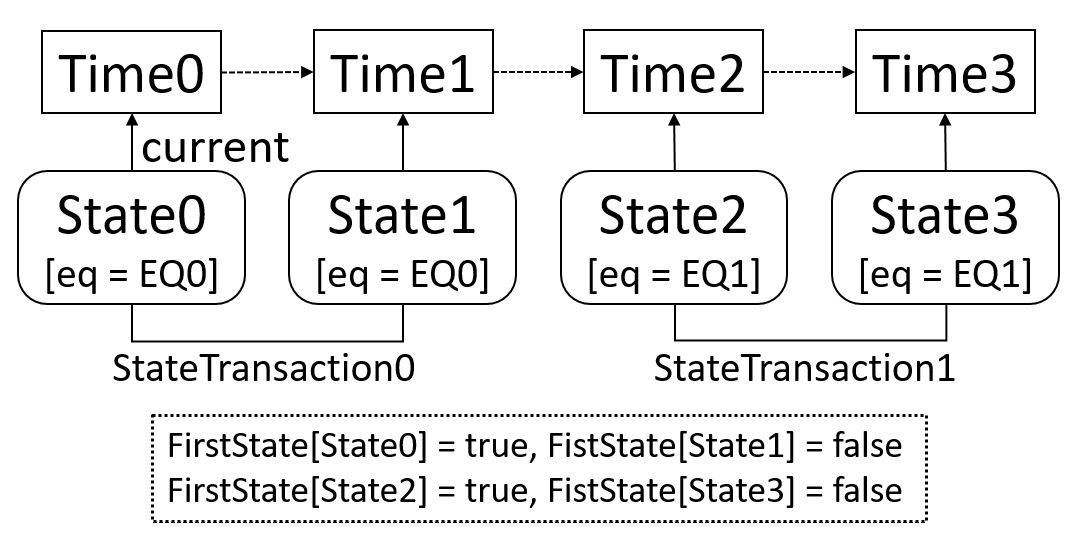
\includegraphics[width=400pt]{./fig/InitialState.eps}
\caption{InitialStateの動作例}
\label{fig:InitialState}
\end{figure}

\end{document}
